\documentclass[tikz]{standalone}
\begin{document}
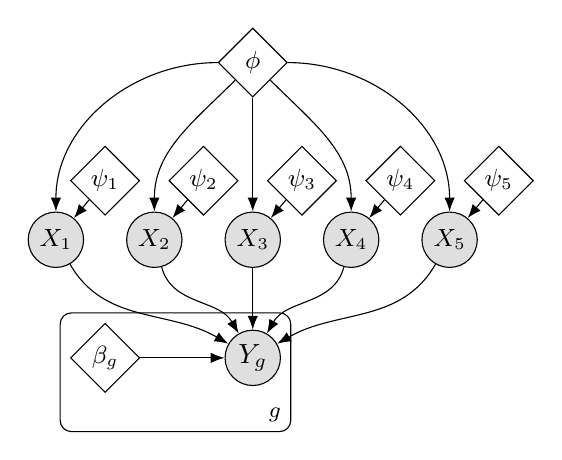
\begin{tikzpicture}

\usetikzlibrary{bayesnet, arrows.meta}

\newlength{\xdist}
\setlength{\xdist}{1.25cm}
\newlength{\ydist}
\setlength{\ydist}{1.5cm}

%\path (-4,-4) grid (4,4);

% styles
\pgfkeys{/tikz/every path/.style={->, -{Latex[length=5pt]}}} % draw arrowheads
\pgfkeys{/var/.style={draw, node font=\small}} % base style for variables
\pgfkeys{/mydet/.style={/var, inner sep=0, diamond, minimum size=25pt}} % detarministic variables
\pgfkeys{/myrnd/.style={/var, inner sep=0, circle, minimum size=20pt}} % latent variables
\pgfkeys{/myobs/.style={fill=gray!25}} % observed variables
\pgfkeys{/mylat/.style={}} % latent variables

% obsolete styles
\pgfkeys{/tech/.style={fill=blue!50!white}}
\pgfkeys{/biol/.style={fill=green}}
\pgfkeys{/response/.style={fill=gray, /myrnd}}
\pgfkeys{/param/.style={fill=pink}}

% main row of X_j
\coordinate (x1) at (-2.0\xdist,1\ydist);
\coordinate (x2) at (-1.0\xdist,1\ydist);
\coordinate (x3) at (0.0\xdist,1\ydist);
\coordinate (x4) at (1.0\xdist,1\ydist);
\coordinate (x5) at (2.0\xdist,1\ydist);
% additional, upper row for interaction terms or X_j specific parameters
\path foreach \j in {1,...,5} {
(x\j) +(0.5\xdist,0.5\ydist) coordinate (xx\j)
};
% response
\node[obs] (y) at (0,0) {\(Y_g\)};


% set styles
\pgfkeys{/x/.style={/myobs, /myrnd}}
\pgfkeys{/xx/.style={/mylat, /mydet}}
\pgfkeys{/beta/.style={/mylat, /mydet}}
\newcommand{\X}[0]{X}
\newcommand{\XX}[0]{\psi}

\coordinate (beta) at (-1.5\xdist,0.0\ydist);
\foreach \j in {1,...,5} {
\node[/x] (X\j) at (x\j) {\(\X_\j\)}; % X_
}


% beta and plate
\node[/beta] (betag) at (beta) {\(\beta_g\)};
\plate {v-plate} {(y) (betag)} {\(g\)};
\draw (betag) -- (y); % dependence of X_j on each psi_j

% top group
\node[/mylat, /mydet] (top) at (0.0\xdist,2.5\ydist) {\(\phi\)};
\foreach \j in {1,...,5} {
\node[/xx] (XX\j) at (xx\j) {\(\XX_\j\)}; % place psi_j
\draw (XX\j) -- (X\j); % dependence of X_j on each psi_j
\draw (top) to[out=-225 + 45 * \j,in=90] (X\j); % dependence of X_j on phi
\draw (X\j) to[out=-45 - 15 * \j, in=180 - 30 * \j] (y); % dependence of Y on each X_j
}

\end{tikzpicture}
\end{document}
